    Este problema fue abordado en un inicio por Paul Dirac en los primeros años de la mecánica cuántica. Sin embargo, su propuesta de un operador de fase cuántica se demostró que poseía bastantes inconsistencias matemáticas. Posterior a Dirac varios científicos abordaron el problema de diferentes maneras en esta sección vamos a abordar el formalismo de Dirac y Susskind-Glogower y nuestra solución al problema mediante el formalismo de Fourier Fraccionario.
    
\section{La fase de Dirac}

        Para entender la propuesta de Dirac vamos a aproximarnos desde un régimen clásico, planteando campos y a partir definir operadores. Consideremos la cavidad mostrada en la figura \ref{fig:cavidad}. Clásicamente el vector de campo eléctrico $\vec{E}(\vec{r},t)$ puede ser expandido como una superposición de ondas planas cada una caracterizada por un vector de onda $\vec{k}$ y vector de polarización $\hat{e}_{k}$. Por conveniencia vamos a limitar el desarrollo a un campo linealmente polarizado con una sola frecuencia. Esta suposición permite tratar el campo eléctrico mediante una descomposición del tipo

        \begin{equation}
            \vec{E}(\vec{r},t) = \left( \frac{\hbar \omega}{2\epsilon_0 L^3} \right)^{1/2} \sum_k \left[a_k e^{i(\vec{k}\cdot \vec{r} - \omega t)} + a_k^* e^{-i( \vec{k}\cdot \vec{r} - \omega t )}  \right],
        \end{equation}

        donde $\omega$ es la frecuencia angular y $\epsilon_0$ es la permitividad eléctrica en el vacío. El conjunto de vectores de onda $\{\vec{k_i}\}$ en la expansión está determinada por las condiciones de fronteras de la onda electromagnética dentro de la cavidad \ref{fig:cavidad}. Si acotamos las condiciones a un campo monomodal, es decir, tenemos un solo vector de onda $\vec{k}=\vec{k}_0$ y se pierde la dependencia de $\vec{k}$ de $a_k$, entonces 

        \begin{equation}
            \vec{E}(\vec{r},t) = \left( \frac{\hbar \omega}{2\epsilon_0 L^3} \right)^{1/2} \left[ ae^{i( \vec{k}\cdot\vec{r} - \omega t )} + a^* e^{-i ( \vec{k}\cdot \vec{r} - \omega t )} \right].
        \end{equation}

        El uso de $a$ es una conveniencia, puesto que no representa nada más que la amplitud adimensional del campo eléctrico, medida en unidades del campo por cuanto $\left(\hbar\omega/2\epsilon_{0}L^{3}\right)^{1/2}$, y su utilidad radica en el papel que juega a la hora de definir los operadores de creación y destrucción. Siguiendo este desarrollo, como $a$ es un número complejo, este se puede expresar en su forma polar como $a = re^{i\phi}$, por lo que la expresión del campo eléctrico se reduce a 

        \begin{equation}
            \vec{E}(\vec{r},t) = \vec{E}_0 \cos\left( \vec{k}_0\cdot \vec{r} - \omega t + \phi \right),\quad \text{donde} \quad \vec{E}_0 = \left( \frac{2\hbar \omega}{\epsilon_0 L^3} \right)^{1/2}r \hat{e},
        \end{equation}
        la cual es la descomposición clásica de amplitud $E_0$ y fase $\phi$.

        Tomando los campos como operadores y definiendo los operadores de creación y aniquilación que satisfacen la relación de conmutación $\left[ \hat{a}, \hat{a}^\dagger \right] = 1$. Debido a que las cantidades en mecánica cuántica son operadores y no números complejos, la descomposición en amplitud y fase no es viable, de hecho, se convierte en un problema realmente difícil. 

        Para abordar el formalismo de Dirac, vamos a partir de la composición polar de las amplitudes clásicas $a = Re^{i\phi}$ en donde se puede despejar al exponencial de fase como $e^{i\phi} = a/R$. De manera análoga, Dirac planteó una descomposición polar para el exponencial de fase como sigue

        \begin{equation}
            e^{i\hat{\phi}} = \hat{a} \hat{R}^{-1},
        \end{equation}
        asumiendo que $e^{i\phi}$ es un exponencial de fase, donde asumiremos que el operador de fase $\hat{\phi}$ es hermítico, y que la amplitud $\hat{R}$ es también un operador hermítico, por ende tenemos que el operador de creación se escribe como

        \begin{equation}
            \hat{a}^{\dagger} = \left( e^{i\hat{\phi}} \hat{R} \right)^\dagger = \hat{R}e^{-i\hat{\phi}},
        \end{equation}
        con esto en cuenta, podemos encontrar la relación entre $\hat{R}$ y el operador número $\hat{N}$ como sigue

        \begin{equation}
            \hat{a}^\dagger\hat{a} = \hat{N} = \hat{R} e^{-i\hat{\phi}}e^{i\hat{\phi}}\hat{R} = \hat{R}^2 \rightarrow \hat{R} = \hat{N}^{1/2}.
        \end{equation}
        Con esto en cuenta el operador exponencial de fase de Dirac se define como 

        \begin{equation}\label{eq:ExpDirac}
            e^{i\hat{\phi}} = \hat{a}\hat{N}^{-1/2}.
        \end{equation}

        Para darnos cuenta de los problemas de este operador de exponencial de fase \ref{eq:ExpDirac} vamos a encontrar las relaciones de conmutación fundamentales relacionados a este operador. Primero la relación de conmutación entre el exponencial de fase y el operador número

        \begin{align}
            & \left[ e^{i\hat{\phi}}, \hat{N} \right] = e^{i\hat{\phi}}\hat{N} - \hat{N}e^{i\hat{\phi}} = e^{i\hat{\phi}}\hat{N} - \hat{a}^\dagger\hat{a} \hat{a} \hat{N}^{-1/2},\\
            & \left[ e^{i\hat{\phi}}, \hat{N} \right] = e^{i\hat{\phi}}\hat{N} - \left( \hat{a}\hat{a}^\dagger -1 \right)\hat{a}\hat{N}^{-1/2} = e^{i\hat{\phi}}\hat{N}- \hat{a}\hat{N}\hat{N}^{-1/2} + \hat{a}\hat{N}^{-1/2},\\
            & \left[ e^{i\hat{\phi}}, \hat{N} \right] = e^{i\hat{\phi}}\hat{N} - e^{i\hat{\phi}}\hat{N} + e^{i\hat{\phi}},\\
            & \left[ e^{i\hat{\phi}}, \hat{N} \right] = e^{i\hat{\phi}},
        \end{align}
        usualmente conocido como el criterio de Lerner. A partir de la relación de conmutación  $\left[ e^{i\hat{\phi}}, \hat{N} \right] = e^{i\hat{\phi}}$ podemos obtener la relación de conmmutación entre $\hat{N},\hat{\phi}$, para ello, usamos el siguiente teorema; dados $\hat{A},\hat{B}$ dos operadores, y $f$ algún funcional diferenciable, se tiene que

        \begin{equation}
            \left[\hat{A},f\left( \hat{B} \right)\right] = \frac{\partial f}{\partial \hat{B}} [\hat{A},\hat{B}].
        \end{equation}
        Si tomamos a $\hat{A}=\hat{N}$ y a $\hat{B}=e^{i\hat{\phi}}$ tendremos el siguiente resultado

        \begin{align}\label{eq:ComNPhi}
            & \left[ \hat{N}, e^{i\hat{\phi}} \right] = ie^{i\hat{\phi}}\left[\hat{N},\hat{\phi} \right] = -e^{i\hat{\phi}},\\
            & \left[\hat{N}, \hat{\phi}\right] = i.
        \end{align}
        Esta relación de conmutación lo que muestra que el operador número $\hat{N}$ y el operador de fase $\hat{\phi}$ son pares canónicamente  conjugados, (cabe recalcar que no aparece $\hbar$ debido a que el operador número y el operador de fase son adimensionales). Esta ecuación, inmediatamente nos lleva a una relación de incertidumbre la cual es frecuentemente vista en discusiones fenomenológicas en las fluctuaciones del número y fase del campo óptico

        \begin{align}
            & \Delta \hat{N}\, \Delta \hat{\phi} \geq \frac{1}{2}\left| \left\langle [\hat{N},\hat{\phi}]\right\rangle \right| = \frac{1}{2}.
        \end{align}

        Hasta el momento todo parece correcto y bien direccionado, sin embargo, en todo el desarrollo previo surgen varios errores. Por ejemplo, si tomamos los elementos de matriz del conmutador \ref{eq:ComNPhi} en la base de los estados número $\ket{n},\ket{n'}$, donde $\hat{N}\ket{n'}=N'\ket{n'}$ tendremos

        \begin{align}
            & \bra{n}\left( \hat{N}\hat{\phi} - \hat{\phi}\hat{N} \right) \ket{n'} = i \braket{n|n'} ,\\
            & (n-n')\bra{n}\hat{\phi}\ket{n'} = i \delta_{nn'}.
        \end{align}
        Para $n=n'$ se llega a una singularidad, a una ecuación $0=i$. Susskind y Glogower también demostraron que el exponencial de fase definido por Dirac no es un operador unitario, y la raíz del problema está en que $\hat{N}^{-1/2}$ no está definido sobre el estado de vacío, pues $\hat{N}\ket{0} = 0$. Adoptando la convención natural de que $\hat{N}^{-1/2}\ket{0}=0$, los dos productos resultan distintos,
        \begin{align}
            & e^{i\hat{\phi}}e^{-i\hat{\phi}} = \hat{a}\hat{N}^{-1/2} \hat{N}^{-1/2}\hat{a}^\dagger = \hat{a}\hat{N}^{-1}\hat{a}^\dagger = \mathbb{I},\\
            & e^{-i\hat{\phi}}e^{i\hat{\phi}} = \hat{N}^{-1/2}\hat{a}^\dagger\hat{a}\hat{N}^{-1/2} = \hat{N}^{-1/2}\hat{N}\hat{N}^{-1/2}= \mathbb{I} - \ket{0}\bra{0},
        \end{align}
        donde el primero sí reproduce la identidad, porque $\hat{a}^{\dagger}$ saca al estado del vacío antes de que actúe $\hat{N}^{-1}$, mientras que el segundo falla precisamente sobre $\ket{0}$. \textbf{La no unitariedad del exponencial de fase de Dirac se concentra por completo en el estado de vacío}, y esa es la razón por la cual no existe un operador hermítico $\hat{\phi}$ del cual $e^{i\hat{\phi}}$ sea la exponencial.

        \begin{figure}[htbp]
            \centering
            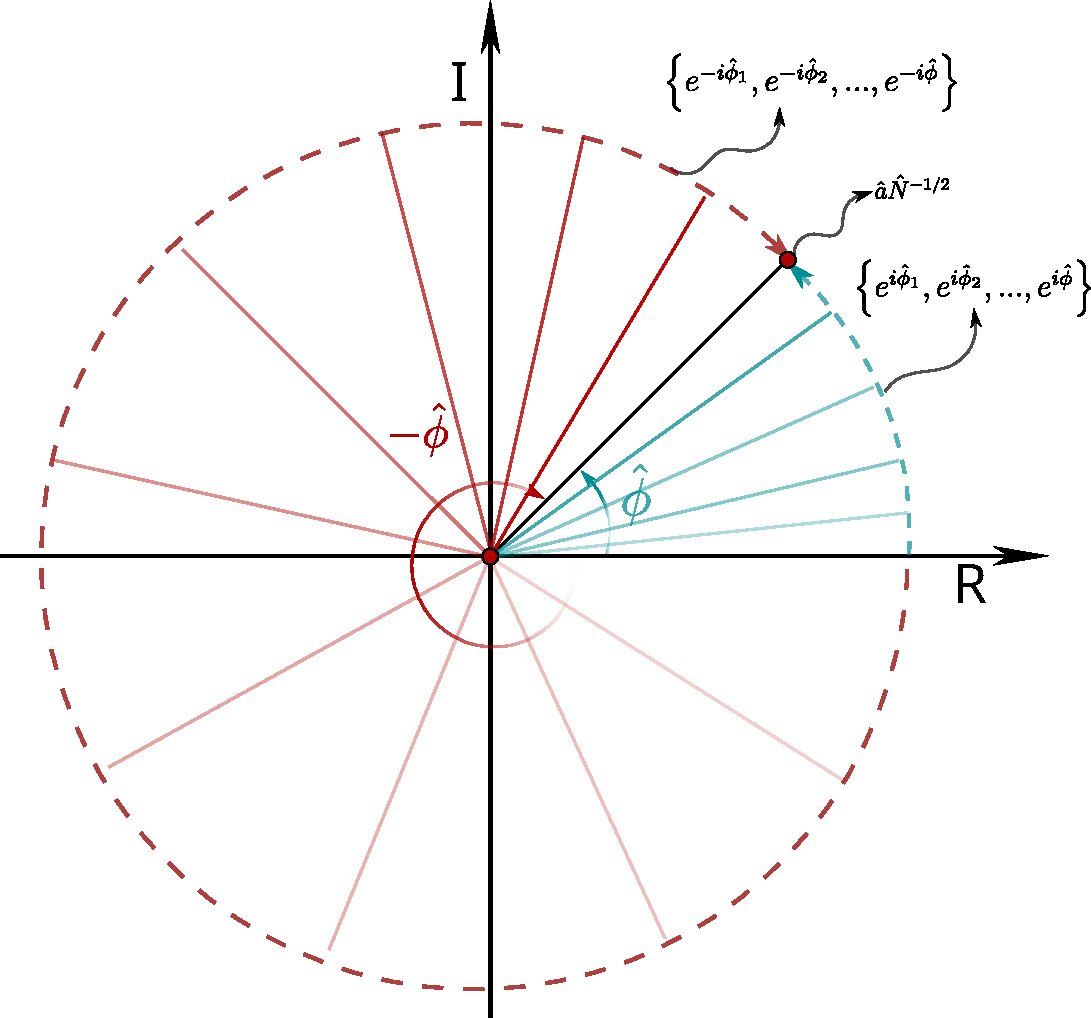
\includegraphics[width=0.7\linewidth]{Capitulo 7/Figuras/FaseDirac.pdf}
            \caption{Representación esquemática sobre el plano complejo $\mathbb{C}^2$ en el cual se ve el efecto del exponencial de fase $e^{i\hat{\phi}}$ y de su adjunto
            $e^{-i\hat{\phi}}$.}
            \label{fig:FaseDirac}
        \end{figure}
        
        Antes de seguir abordando los problemas de la fase de Dirac demos algo de sentido geométrico a la no unitaridad del operador exponencial de fase. En la figura \ref{fig:FaseDirac} se representa esquemáticamente distintas rotaciones sobre el plano complejo $\mathbb{C}^2$ que representa el exponencial de fase $e^{i\hat{\phi}}$ de color azul, en donde se sigue la convención de rotaciones en sentido antihorario mientras que de color rojo se representan las rotaciones relacionado al operador $e^{-i\hat{\phi}}$. Cuando trabajamos sobre el cuerpo de los números complejos se tiene que todo complejo $z \in \mathbb{C}$ tiene una representación polar en donde el exponencial de fase satisface que es unitario pero, esta propiedad viene heredada de la naturaleza conmutativa de $\mathbb{C}$ acá hemos demostrado \ref{eq:ComNPhi} que no hay conmutación, por ende, es natural que el exponencial de fase propuesto por Dirac no sea unitario, ambos representan procesos físicos distintos como se trata de ilustrar en la figura \ref{fig:FaseDirac}.

        Los problemas del formalismo de Dirac se pueden identificar de dos fuentes. La primera es que el espectro de $n$ no se extiende a valores negativos, sino que solo por los enteros no negativos desde $0$ hasta $+\infty$. Para entender un poco esto vamos a ver el desarrollo de Barnett y Pegg e introducir estados número negativos, tal que podemos escribir la siguiente expresión

        \begin{equation}
            e^{i\hat{\phi}} = \sum_{n=-\infty}^{\infty} \ket{n}\bra{n+1},
        \end{equation}
        y es fácil ver que el adjunto conjugado es el operador
        \begin{equation}
            e^{-i\hat{\phi}} = \sum_{n=-\infty}^{\infty}\ket{n+1}\bra{n},
        \end{equation}
        en donde podemos verificar que este exponencial de fase es unitario

        \begin{align}\label{eq:Pegg}
            &e^{i\hat{\phi}}e^{-i\hat{\phi}} = \sum_{n,n'=-\infty}^{\infty} \ket{n}\braket{n+1|n'+1}\bra{n'} = \sum_{n,n'=-\infty}^{\infty}\ket{n}\delta_{nn'}\bra{n'} = \sum_{n=-\infty}^\infty\ket{n}\bra{n}= \mathbb{I},\\
            & e^{-i\hat{\phi}}e^{i\hat{\phi}} = \sum_{n,n'=-\infty}^{\infty}\ket{n+1}\braket{n|n'}\bra{n'+1} = \sum_{n,n'=-\infty}^{\infty}\ket{n+1}\delta_{nn'}\bra{n+1} = \sum_{n=-\infty}^{\infty}\ket{n+1}\bra{n+1}= \mathbb{I}
        \end{align}

        Vale la pena notar que los estados número negativos son solamente una herramienta matemática que permite definir un operador unitario pero no tienen sentido físico. Así como Barnett y Pegg mencionaron "... la deducción de los estados propios del oscilador armónico se requiere un estado base que es aniquilado por el operador de aniquilación tal que el espectro de energía es acotado desde abajo... Estados de energía negativa no están excluidos pero ellos deben desprenderse de los estados de base de energía positiva que son aniquilados por el operador de aniquilación... Estados que contienen un número negativo de fotones son inaccesibles a un sistema físico, por lo tanto, su mera existencia en el formalismo no predice ningún fenómeno nuevo en la electrodinámica cuántica".

        Debido a que $e^{i\hat{\phi}}$ es un operador unitario este define un operador hermítico $\hat{\phi}$. De la ecuación \ref{eq:Pegg} se puede deducir un conmutador como el de la regla de Lerner

        \begin{equation}
            \left[ e^{i\hat{\phi}},\hat{N} \right] = e^{i\hat{\phi}},
        \end{equation}
        que de manera análoga nos lleva a la conmutación canónica entre $\hat{N},\hat{\phi}$ y se repite el problema de tener una ecuación singular del tipo $0=i$ como pasó con el exponencial de Dirac.

        La fuente de problemas restante se debe a que $\hat{\phi}$ es un operador de ángulo. Esto se puede apreciar mejor al comparar este tratamiento de fase y número con algún problema análogo, como el momento angular y su variable conjugada. En esta analogía, el operador de momento angular $\hat{L}$, entendido como cualquiera de sus componentes, hace el papel del operador número. Sin embargo, como se vio, la introducción de estados número negativos es una herramienta matemática más no física, entonces los valores propios de $\hat{L}$ pertenecientes al estado propio $\ket{m}$ realmente generan el rango de enteros que van desde $-\infty$ hasta $\infty$. Vamos a asumir que $\hat{L}$ y su ángulo canónicamente conjugado $\hat{\chi}$ satisfacen la relación de conmutación

        \begin{equation}
            \left[ \hat{L},\hat{\chi} \right] = i.
        \end{equation}

        En la base de $\chi$ los operadores toman la forma $\hat{\chi}\to \chi$ y $\hat{L}\to -i\frac{\partial}{\partial\chi}$. Las funciones propias de $\hat{L}$, $\braket{\chi|m}$, son simplemente proporcionales a $e^{im\chi}$. $m$ se convierte en un valor entero después de imponer la condición de que $\chi \to \chi + 2\pi$. En este orden de ideas, las funciones propias base son periódicas, con periodos de $2\pi$. Sin embargo, debemos restringir el rango de $\chi$, puesto que este cubre a todo $\mathbb{R}.$

        \begin{figure}[htbp]
            \centering
            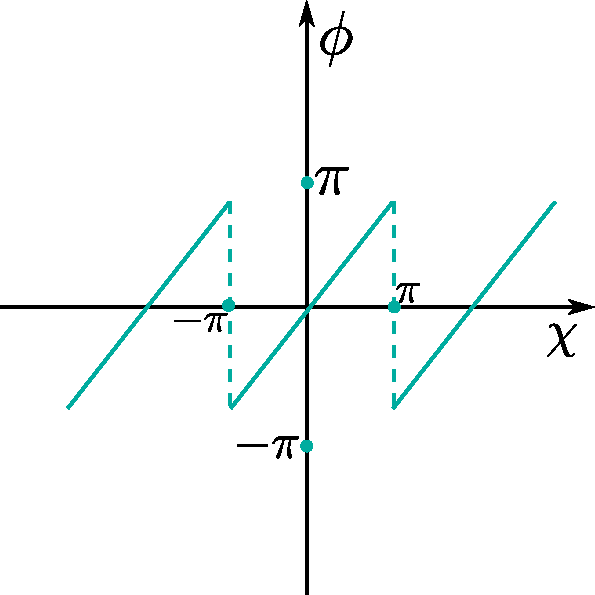
\includegraphics[width=0.5\linewidth]{Capitulo 7/Figuras/chivsphi.pdf}
            \caption{Relación entre el operador de ángulo restringido $\hat{\phi}$ con $-\pi < \hat{\phi} \leq \pi$ y el operador de ángulo $\hat{\chi}$.}
            \label{fig:chivsphi}
        \end{figure}

        Un resultado de esto es que $\hat{\chi}$ opera impropiamente sobre el espacio de las funciones propias, a pesar de que $\braket{\chi|m}$ es periódico en $\chi$, $\hat{\chi}\braket{\chi|m}$ no lo es. Una forma de salir de este problema es introduciendo un ángulo $\phi$ relacionado con $\chi$, el cual es periódico. Si escogemos el intervalo de periodicidad de manera arbitraria, como por ejemplo, $-\pi$ a $\pi$, entonces la relación entre $\hat{\chi}$ y $\hat{\phi}$ se muestra en la figura \ref{fig:chivsphi}.

        Volviendo al conmutador, recordando que el operador $\hat{L}$ es una derivada parcial y recordando las discontinuidades que hay en la relación de $\phi vs \chi$ esta da lugar a una función delta de Dirac, por ende tenemos

        \begin{equation}\label{eq:phires}
            \left[ \hat{L},\hat{\phi} \right] = i - 2\pi i \delta(\phi-\pi), \quad -\pi < \phi \leq \pi. 
        \end{equation}

        El mismo argumento aplica a la relación de conmutación $[\hat{N},\hat{\phi}]$ ya que esta es isomorfa a la conmutación $[\hat{L},\hat{\phi}]$ en donde el espectro de $n$ se extiende a valores negativos. Con esta relación de conmutación \ref{eq:phires}, si calculamos los elementos de matiz en la base de los estados número tendremos ahora

        \begin{equation}
            \bra{n} \left( \hat{N}\hat{\phi} - \hat{\phi}\hat{N} \right) \ket{n'} = i \left[ 1 - 2\pi \bra{n}\delta(\phi-\pi) \ket{n'} \right].
        \end{equation}
        Recordemos que $\braket{\phi|n}\propto e^{in\phi}$ en esta representación, entonces tenemos

        \begin{equation}
            (n-n')\bra{n}\hat{\phi}\ket{n'} = i \left[ 1 - e^{i(n'-n)\pi} \right],
        \end{equation}
        la cual es una relación matemáticamente consistente.

        Al revisar la discusión hasta ahora, se observa que el formalismo de Dirac sufre de dos dificultades. Primero, la resolución del operador de campo en componentes de amplitud y fase produce un operador no unitario, $e^{i\hat{\phi}}$, por lo que esta expresión no define un operador hermítico $\hat{\phi}$. El origen de este problema se debe a que el espectro del operador número, $\hat{n}$, está acotado inferiormente. Esta es una dificultad importante del formalismo de Dirac.

        Suponiendo que se pudiera resolver esta dificultad, se encuentra que al tener el número y la fase conjugados canónicamente (es decir, la ecuación \ref{eq:ComNPhi}, $[\hat{n},\hat{\phi}]=i$), se obtienen resultados matemáticamente inconsistentes. Sin embargo, como hemos visto, la fuente de este problema particular es fácilmente rastreable a descuidos en el manejo del dominio de $\hat{\phi}$. Un tratamiento adecuado de este aspecto del operador fase produce la relación de conmutación modificada,  equivalente a la ecuación \ref{eq:phires}, que se reduce a la forma canónica $[\hat{n},\hat{\phi}]=i$ excepto en un límite del dominio de $\hat{\phi}$. Por lo tanto, esto es solo un problema relativamente menor, aunque potencialmente problemático si no se maneja correctamente. En la siguiente sección consideraremos un intento temprano de modificar la teoría de Dirac para evitar esta segunda dificultad, lo que da lugar al llamado formalismo de Susskind–Glogower.

\section{El formalismo de Susskind-Glogower}

	    Como se ha visto, el enfoque de Dirac para el problema del operador fase sufre de una inconsistencia matemática relacionada con el dominio del operador. Louisell (1963) sugirió que esto podría evitarse trabajando con funciones periódicas del operador, en lugar del operador mismo.
	
	    Susskind y Glogower (1964) siguieron esta sugerencia y desarrollaron una teoría funcional (aunque difícil de usar) con algunos problemas formales residuales. La teoría ha evolucionado hasta convertirse en un formalismo estándar, utilizado constantemente hasta la actualidad. Por lo tanto, vale la pena examinar en detalle el trabajo de Susskind-Glogower.
	    
	    Aunque la sugerencia de Louisell y su implementación por Susskind-Glogower llevan a examinar objetos como $\cos\hat{\phi}$, $\sin\hat{\phi}$ y $\mathrm{e}^{\mathrm{i}\hat{\phi}}$, se encuentra que este último operador exponencial no es unitario. Por consiguiente, $\mathrm{e}^{\mathrm{i}\hat{\phi}}$ no puede ser una función de un operador hermítico $\hat{\phi}$, lo que indica que debe tenerse cuidado con estos objetos. Así, para evitar ser inducidos a razonamientos erróneos, seguiremos libremente a Carruthers y Nieto  y usaremos la notación sugerente, manejable y menos propensa a errores $\hat{C}$, $\hat{S}$ y $\hat{E}$ para estos operadores.
	
	    Susskind y Glogower definen los operadores de exponencial de fase en conexión con el operador de aniquilación $\hat{a}$ como
	
	    \begin{equation}\label{eq:SGE}
	        \hat{E} = \left( \hat{N}+1 \right)^{-1/2}\hat{a}, \quad\hat{E}^\dagger = \hat{a}^\dagger \left( \hat{N}+1 \right)^{-1/2},
	    \end{equation}
	    la razón por la cual se escoge el operador número más uno no es del todo clara, sin embargo, podemos hacer una deducción de este operador desde la teoría electromagnética clásica. Partamos la amplitud de campo eléctrico $a = Re^{i\phi}$, donde, como ya vimos, se puede despejar al exponencial de fase como $e^{i\phi}=R^{-1}a$, elevando a estatuto de operador y suponiendo que $\hat{\phi}, \hat{R}$ son operadores hermíticos tendremos las siguientes ecuaciones
	
	    \begin{align}
	        & \hat{a}\hat{a}^\dagger = \hat{R}e^{i\hat{\phi}}e^{-i\hat{\phi}}\hat{R} = \hat{R}^2,
	    \end{align}
	    ahora, debemos hacer uso del conmutador $[\hat{a},\hat{a}^\dagger]=1$ para obtener el siguiente resultado
	
	    \begin{equation}
	        \hat{a}\hat{a}^\dagger= \hat{a}^\dagger\hat{a}
	        +1=\hat{N}+1 = \hat{R}^2, 
	    \end{equation}
	    de donde es fácil obtener que $\hat{R}= \sqrt{\hat{N}+1}$. De esta manera, tomando al operador $\hat{E}$ como el análogo operador exponencial de fase $e^{i\hat{\phi}}$ llegamos a los operadores de Susskind y Glogower \ref{eq:SGE}. Con base en este operador exponencial de fase se pueden definir los operadores $\hat{C},\hat{S}$ equivalentes al coseno y seno, respectivamente, de la siguiente manera
	
	    \begin{equation}
	        \hat{C} = \frac{1}{2}\left( \hat{E}+\hat{E}^\dagger \right),\quad \hat{S}= \frac{1}{2i}\left( \hat{E}-\hat{E}^\dagger \right).
	    \end{equation}
	
	    Si usamos la base de los estados número, podemos expresar a los operadores $\hat{E},\hat{E}^\dagger$ en términos de estos, para ello tomaremos las expresiones \ref{eq:SGE} y usaremos el hecho de que de $\{\ket{n}\}$ genera un espacio de Hilbert, es decir, un espacio completo
	
	    \begin{align}\label{eq:SGNum}
	        & \hat{E} =  \sum_{n=0}^{\infty}   \ket{n} \bra{n} \left( \hat{N}+1 \right)^{-1/2}\hat{a} = \sum_{n=0}^\infty \ket{n} \left( n+1 \right)^{-1/2} \bra{n}\hat{a} = \sum_{n=0}^\infty \ket{n}\bra{n+1},\\
	        & \hat{E}^\dagger = \left(  \sum_{n=0}^\infty \ket{n}\bra{n+1}\right)^\dagger = \sum_{{n=0}}^\infty \ket{n+1}\bra{n}.
	    \end{align}
	
	    Si nos fijamos, estos operadores de exponencial de fase son casi idénticos a los propuestos por Barnett y Pegg, sin embargo, estos no tienen el problema de un espectro de estados número negativos, sin embargo, mientras que el operador de Barnett y Pegg son unitario, el de Susskind-Glogower es un operador semi-unitario, esto se ve de la siguiente manera
	
	    \begin{align}\label{eq:SGUni}
	        & \hat{E}\hat{E}^\dagger = \sum_{n,n'=0}^{\infty} \ket{n}\braket{n+1|n'+1}\bra{n'} = \sum_{n,n'=0}^\infty\ket{n}\delta_{nn'}\bra{n'} = \sum_{n=0}^\infty \ket{n}\bra{n}=\mathbb{I},\\
	        & \hat{E}^\dagger\hat{E} = \sum_{n,n'=0}^\infty \ket{n+1}\braket{n|n'}\bra{n'+1} = \sum_{n=0}^\infty \ket{n+1}\bra{n+1} = \mathbb{I}- \ket{0}\bra{0}.
	    \end{align}
	
	    El proyector sobre el estado de vacío $\ket{0}\bra{0}$ es el que evita la unitaridad del operador $\hat{E}$. Esto sugiere que en estados de campo con un número de fotones grande en promedio, es decir, $\bar{N} = \braket{\hat{n}}\gg  1$, la componente del vacío cuántico será muy pequeña, y el comportamiento de $\hat{E}$ es aproximadamente unitario. Si tomamos la representación gráfica \ref{fig:FaseDirac} lo que podemos interpretar que sucede es que al completar un ángulo $\phi$ ya sea en un sentido horario o una antihorario hay fluctuaciones del vacío cuántico naturales, el vacío cuántico está constantemente fluctuando por ende, para un operador de exponencial de fase puro este mantendrá un cierto ancho de banda sobre el ángulo barrido. Usando el resultado de \ref{eq:SGUni} podemos llegar a las relaciones de conmutación de los operados de seno, coseno y número de la siguiente manera
	
	    \begin{align}
	        & \left[ \hat{C},\hat{N} \right] = i \hat{S},\\
	        & \left[ \hat{S},\hat{N} \right] = -i\hat{C},\\
	        & \left[ \hat{C},\hat{S} \right] = \frac{1}{2}i \ket{0}\bra{0},\\
	        & \hat{C}^2+\hat{S}^2 = 1 - \frac{1}{2}\ket{0}\bra{0}.
	    \end{align}
	
	    Es realmente interesante ver cómo el proyector sobre el estado de vacío, es decir, el vacío cuántico, impide las conmutaciones entre el seno y el coseno y a su vez, impide la aparición de la identidad de Pitágoras.
	
	    Las funciones propias del operador $\hat{E}$ son $\ket{e^{i\phi}}$ y satisfacen la ecuación
	
	    \begin{equation}
	        \hat{E}\ket{e^{i\phi}} = e^{i\phi}\ket{e^{i\phi}},
	    \end{equation}
	    las cuales son de gran interés general en la teoría de operadores. Estas funciones propias se pueden escribir en la base de los estados número como
	
	    \begin{equation}
	        \ket{e^{i\phi}} = \sum_{n=0}^\infty e^{in\phi}\ket{n}.
	    \end{equation}
	
	    Estos estados, con un factor de normalización diferente, fueron utilizados temprano en la historia de la mecánica cuántica por London. Los estados $\ket{e^{i\phi}}$ forman un conjunto completo, dando paso a una relación de clausura como sigue
	
	    \begin{equation}
	        \frac{1}{2\pi} \int_{-\pi}^\pi \ket{e^{i\phi}}\bra{e^{i\phi}}d\phi = \mathbb{I}.
	    \end{equation}

    Ahora vamos a analizar los valores esperados de los operadores en los estados coherentes $\ket{\alpha}$. Si escribimos al parámetro complejo $\alpha$ como $\alpha=re^{i\theta}$ y usando la expansión de los estados coherentes de Glauber en la base de los estados número

    \begin{equation}
        \ket{\alpha} = e^{-\frac{|\alpha|^2}{2}}\sum_{n=0}^\infty \frac{\alpha^n}{\sqrt{n!}}\ket{n},
    \end{equation}
    uno puede obtener todas las siguientes expresiones 

    \begin{align}
        & \bra{\alpha}\hat{C}\ket{\alpha} = re^{-r^2}\psi_1(r)\cos\theta,\\
        &\bra{\alpha}\hat{S}\ket{\alpha} = re^{-r^2}\psi_1(r)\sin\theta,\\
        & \bra{\alpha}\hat{C}^2\ket{\alpha} = \frac{1}{2}-\frac{1}{4}e^{-r^2} + \frac{1}{2}r^2e^{-r^2}\psi_2(r)\cos 2\theta,\\
        & \bra{\alpha}\hat{S}^2\ket{\alpha}= \frac{1}{2}-\frac{1}{4}e^{-r^2} - \frac{1}{2}r^2e^{-r^2}\psi_2(r)\cos 2\theta,\\
        & \bra{\alpha} \hat{C}^2+  \hat{S}^2 \ket{\alpha} = 1 - \frac{1}{2}e^{-r^2},\\
        & \bra{\alpha}\hat{C}^2 - \hat{S}^2 \ket{\alpha} = r^2e^{-r^2}\psi_2(r)\cos 2\theta,\\
        & \bra{\alpha}\hat{C}\hat{S} + \hat{S}\hat{C}\ket{\alpha} = r^2 e^{-r^2}\psi_2 (r)\sin 2\theta,\\
        & \bra{\alpha} \hat{C}\hat{S}- \hat{S}\hat{C} \ket{\alpha} = \frac{1}{2}ie^{-r^2},
    \end{align}
    donde
    \begin{equation}
        \psi_1(r) = \sum_{n=0}^\infty \frac{r^{2n}}{n!\sqrt{n+1}}, \quad \psi_2(r) = \sum_{n=0}^\infty \frac{r^{2n}}{n!\sqrt{(n+1)(n+2)}},
    \end{equation}
    las cuales tienen las siguientes formas asintóticas para $r\gg 1$:

    \begin{align}\label{eq:Asimtotica}
        & \psi_1(r) \to \frac{e^{r^2}}{r}\left[ 1 - \frac{1}{8r^{2}} - \frac{7}{128r^{4}}-\cdots \right],\\
        & \psi_2(r) \to \frac{e^{r^2}}{r}\left[ 1 - \frac{1}{2r^2} + \frac{3}{8r^4}-\cdots \right].
    \end{align}

    El número de fotones medio es $N = \bra{\alpha}\hat{N}\ket{\alpha }=|\alpha|^2 = r^2$. En el límite clásico si $N,r\to\infty$ se usan las expresiones asintóticas \ref{eq:Asimtotica} y todos los valores medios antes mostrados se recuperan como las identidades trigonométricas clásicas bien conocidas.
    
\section{La fase cuántica y la transformación de Fourier Fraccionaria}

    En 1980 Victor Namias demostró que el oscilador armónico cuántico tiene las mismas funciones propias que la transformación de Fourier y, para estudiar el oscilador armónico cuántico propone una generalización de la transformación de Fourier, la cual denominó transformación de Fourier Fraccionaria \cite{namias1980fractional}. Par darle forma al operador de Fourier y al operador de Fourier fraccionaria partamos de la ecuación de valores propios para los estados número y las funciones de Hermite-Gauss $\ket{H_n}$ así

    \begin{equation}
        \mathcal{F}\ket{H_n} = e^{in\frac{\pi}{2}}\ket{H_n} = e^{i\hat{N}\frac{\pi}{2}}\ket{n}.
    \end{equation}

    Para relacionar a los operadores $\hat{N},\mathcal{F}$ vamos a partir del hamiltoniano del oscilador armónico en la base de posición y así despejar al operador número

    \begin{align}
        & \hat{H} = \frac{1}{2}\left( \omega^2\hat{q}^2 + \hat{p}^2 \right) = \frac{1}{2}\left( \omega^2 \hat{x}^2 - \hbar^{2}\partial_{xx} \right) = \hbar\omega \left( \hat{N}+\frac{1}{2} \right),
    \end{align}
    de acá, podemos despejar al operador número como sigue

    \begin{align}
        & \hat{N} = \frac{1}{2\hbar\omega}\left( \omega^2\hat{q}^2 + \hat{p}^2 \right) = \frac{1}{2\hbar\omega}\left( \omega^2 \hat{x}^2 - \hbar^{2}\partial_{xx} \right) - \frac{1}{2},
    \end{align}
    por lo que la ecuación de autovalores para los estados de Hermite-Gauss $\ket{H_n}$ tenemos

    \begin{align}
        & \mathcal{F}\ket{H_n} = e^{i \left[ \frac{1}{2\hbar\omega} \left( \omega^2 \hat{x}^2 - \hbar^{2}\partial_{xx} \right) - \frac{1}{2} \right]\frac{\pi}{2} }\ket{H_n}.
    \end{align}

    Namias identifica al $\frac{\pi}{2}$ como la fase de Fourier del operador $\mathcal{F}_{\pi/2}$ y propone entonces un operador general llamado \textit{transformación de Fourier Fraccionaria} definida por 

    \begin{equation}\label{eq:OpFFR}
        \mathcal{F}_\alpha = e^{i\hat{N}\alpha} = \mathcal{F}_{\pi/2}^a = \left( e^{i\hat{N}\frac{\pi}{2}} \right)^a.
    \end{equation}

    Es fácil ver que el operador de Fourier fraccionario \ref{eq:OpFFR} es unitario, pues satisface $\mathcal{F}^\dagger_\alpha = \mathcal{F}_{-\alpha} = \mathcal{F}^{-1}_\alpha.$ El efecto de la TFF sobre los estados de fase $\ket{\phi}$ definidos por

    \begin{equation}
        \ket{\phi} = \sum_{n=0}^\infty e^{in\phi}\ket{n},
    \end{equation}
    será desarrollado un poco más adelante, así como su efecto sobre los estados coherentes $\ket{\alpha}$ y su relación con la distribución de Wigner.

\section{Efectos de la transformación de Fourier Fraccionaria sobre los estados coherentes y la función de Wigner}

        Para entender el significado o darle interpretación a la TFF vamos a estudiar sus efectos sobre la cuasi-distribución de probabilidad de Wigner. Antes de desarrollar esto vamos a hacer un breve repaso de qué es la función de Wigner.

        La función de Wigner y, en general, las conocidas como funciones $s$-parametrizadas hacen parte de una familia de distribuciones que permiten un mapeo que asocia cada operador a una función (conocida usualmente como símbolo) definida sobre una variedad suave con una estructura matemática muy precisa. Para bien o para mal este mapeo no es único, existe una familia entera de funciones que pueden ser consistentemente asignadas a cada operador. En particular, las \textit{cuasi-distribuciones de probabilidad}, las cuales son bastante útiles en la óptica cuántica, estas son los símbolos correspondientes del operador de densidad $\hat{\rho}=\sum_i p_i \ket{\psi_i}\bra{\psi_i}$. Para variables continuas, como la posición y el momento de un oscilador armónico (en un campo monomodal), las opciones más comunes son las $P$ (Glauber-Sudarshan), $W$ (Wigner) y $Q$ (Husimi) funciones, respectivamente.

        Estas cuasi-distribuciones contienen toda la información acerca del sistema, sin embargo, cada una de ellas corresponde a un ordenamiento diferente de los operadores de creación y destrucción. La representación $P$ es utilizada para evaluar operadores de correlación de campos normalmente ordenadas, la función $Q$ es asociada a un orden anti-normal, y la función de Wigner es empleada con operadores simétricamente ordenados. La función de Wigner ha ganado más peso que cualquiera de las otras ya que, por ejemplo, puede ser reconstruida por tomografía óptica de Homodyne o directamente sampleada por conteo de fotones y, como veremos en esta sección, esta tiene un gran contenido físico y permite dar sentido a muchas relaciones.

        Para construir la función de Wigner supongamos operadores  de cuadratura de posición $\hat{x}$ y momento $\hat{p}$ con una relación de conmutación canónica $[\hat{x},\hat{p}]=i\hbar$, como $\hat{x},\hat{p}$ son operadores no acotados, se va a lidiar con sus contrapartes unitarias 

        \begin{equation}
            \hat{U}(x) = e^{-ix\hat{p}}, \quad \hat{V}(p) = e^{-ip\hat{x}},
        \end{equation}
        los cuales actúan sobre los estados propios de posición $\ket{x}$ y momento $\ket{p}$ como
        \begin{equation}
            \hat{U}(x')\ket{x} = \ket{x+x'}, \quad\hat{V}(p')\ket{p} = \ket{p+p'},
        \end{equation}
        por lo tanto, estos representan desplazamientos a lo largo de los respectivos ejes coordenados. La relación de conmutación se manifiesta en la forma de Weyl como
        \begin{equation}
            \hat{V}(p)\hat{U}(x) = e^{-ixp}\hat{U}(x)\hat{V}(p).
        \end{equation}

        La versión infinitesimal arroja inmediatamente la relación de conmutación estándar, sin embargo, la expresión anterior puede ser más útil.

        En términos de $\hat{U}$ y $\hat{V}$ un operador de desplazamiento general se puede definir como

        \begin{equation}
            \hat{D}(x,p) = e^{ixp/2}\hat{U}(x)\hat{V}(p)= e^{i \left( p\hat{x} - x\hat{p} \right)},
        \end{equation}
        cuyos parámetros $(x,p) \in \mathbb{R}^2$ etiquetan los puntos en el espacio de fase. 

        La transformada de Fourier del operador de desplazamiento $\hat{D}(x,p)$
        \begin{equation}
            \hat{w}(x,p) = \frac{1}{(2\pi)^2}\int_{\mathbb{R}^2} \hat{D}(x',p')  e^{-i \left( px' - xp' \right)}dx'dp',
        \end{equation}
        es una instancia del cuantizador de Stratonovich-Weyl. Este cuantizador puede ser modificado para trabajar, en general, con las cuasi-distribuciones $s$-parametrizadas. Se puede observar que los operadores $\hat{w}(x,p)$ son un conjunto ortonormal que transforma propiamente bajo desplazamientos, es decir

        \begin{equation}
            \hat{w}(x,p) = \hat{D}(x,p) \hat{w}(0,0)\hat{D}^\dagger(x,p),
        \end{equation}
        donde
        \begin{equation}
            \hat{w}(0,0) = \frac{1}{(2\pi)^{2}}\int_{\mathbb{R}^2}\hat{D}(x,p)dxdp = 2 \hat{\mathcal{P}},
        \end{equation}
        y
        \begin{equation}
            \hat{\mathcal{P}} = \int_\mathbb{R} \ket{x}\bra{-x}dx = \int_\mathbb{R}\ket{p}\bra{-p}dp
        \end{equation}
        es el operador de paridad.

        Sea $\hat{A}$ un operador arbitrario de Hilbert-Schmidt\footnote{Un operador de Hilbert-Schmidt es un tipo de operador lineal acotado entre espacios de Hilbert que generaliza el concepto de matrices de dimensión finita a espacios de dimensión infinita.} que actúa sobre el espacio de Hilbert $\mathcal{H}$. Utilizando el cuantizador de Stratonovich-Weyl podemos asociar a $\hat{A}$ una distribución temperada $a(x,p)$\footnote{Una distribución temperada es un elemento del espacio dual $\mathcal{S}'(\mathbb{R}^n)$ de las funciones de Schwartz $\mathcal{S}(\mathbb{R}^n)$ (funciones $C^\infty$ cuyas derivadas de todo orden decaen más rápido que el inverso de cualquier polinomio). Son funcionales lineales continuas que generalizan funciones y medidas, permitiendo transformadas de Fourier en sentido distribucional.} representando la acción de su correspondiente variable dinámica en el espacio de fase. Esta aplicación se conoce como el mapeo de Wigner-Weyl y se escribe como

        \begin{equation}
            a(x,p) = \mathrm{Tr}\left\{ \hat{A}\hat{w}(x,p) \right\}.
        \end{equation}
        La distribución $a(x,p)$ se conoce como el símbolo del operador $\hat{A}$. De manera recíproca, se puede reconstruir el operador a partir de su símbolo como sigue

        \begin{equation}
            \hat{A}=\frac{1}{(2\pi)^2}\int_{\mathbb{R}^2}a(x,p) \hat{w}(x,p)dxdp.
        \end{equation}

        En este contexto, la función de Wigner no es nada más que el símbolo de la matriz de densidad $\hat{\rho}$. Por lo tanto, escribimos
        \begin{align}
            & W_\rho (x,p) = \mathrm{Tr}\left\{ \hat{\rho}\hat{w}(x,p) \right\},\\
            & \hat{\rho} = \frac{1}{(2\pi)^2}\int_\mathbb{R^2}\hat{w}(x,p)W_\rho(x,p)dxdp.
        \end{align}

        Para un estado puro $\ket{\psi}$ la función de Wigner se representa como 

        \begin{equation}
            W_\psi(x,p) =\frac{1}{2\pi} \int_\mathbb{R}\psi(x-x'/2)\psi^*(x+x'/2)e^{ipx'}dx'.
        \end{equation}

        Para ver el efecto de la TFF sobre la función de Wigner vamos a ver primero el efecto de esta sobre los estado coherentes, por el momento, para campos monomodales del oscilador armónico cuántico. Como ya hemos visto, los estados coherentes $\ket{\alpha}$ están dados por
        \begin{equation}
            \ket{\alpha} = e^{-\frac{1}{2}|\alpha|^2} \sum_{n=0}^{\infty} \frac{\alpha^n}{\sqrt{n!}}\ket{n},\quad \alpha = |\alpha|e^{i\theta},
        \end{equation}
        por lo que su TFF es
        \begin{equation}
            \mathcal{F}_\phi \ket{\alpha} = e^{-\frac{1}{2}|\alpha|^2} \sum_{n=0}^{\infty} \frac{\alpha^n}{\sqrt{n!}}e^{i\hat{N}\phi}\ket{n} = e^{-\frac{1}{2}|\alpha|^2} \sum_{n=0}^{\infty} \frac{\alpha^n e^{in\phi} }{\sqrt{n!}}\ket{n}  = \ket{\alpha e^{i\phi}},
        \end{equation}
        y se cumple entonces que al aplicar una transformación de Fourier de orden $\phi$ sobre los estados coherentes se produce un desfase de estos de un ángulo $\phi$. Con esto en mente, el operador de desplazamiento se puede reformular en la forma

        \begin{equation}
            \hat{\mathcal{D}}(\alpha e^{i\phi}) = e^{\alpha e^{i\phi}\hat{a}^\dagger - \alpha^*e^{-i\phi}\hat{a}} = e^{-\frac{1}{2}|\alpha|^2}e^{\alpha e^{i\phi}\hat{a}^\dagger} e^{-\alpha^* e^{-i\phi}\hat{a}}, 
        \end{equation}
        y resulta que el desplazamiento sobre los estados de vacío cuántico $\ket{0}$ se pueden entender en términos de la TFF
        \begin{equation}
            \hat{\mathcal{D}}(\alpha e^{i\phi})\ket{0} = \hat{\mathcal{F}}_\phi\ket{\alpha},
        \end{equation}
        entonces se obtiene la relación $\hat{\mathcal{D}}(\alpha e^{i\phi}) = \hat{\mathcal{F}}_\phi \hat{\mathcal{D}}(\alpha)$. En este orden de ideas, la función característica de Wigner, está dada por

        \begin{equation}
            C_W(\alpha e^{i\phi}) = \mathrm{Tr}\left\{ \hat{\rho}\hat{\mathcal{D}}(\alpha e^{i\phi}) \right\} = \mathrm{Tr} \left\{ \hat{\rho} \hat{\mathcal{F}}_\phi \hat{\mathcal{D}}(\alpha) \right\}
        \end{equation}
        y, finalmente, la función de Wigner  se escribe como

        \begin{equation}
            W\left( \alpha e^{i\phi} \right) = \frac{1}{\pi^2} \int_{\mathbb{C}} e^{\lambda^* \alpha - \lambda\alpha^*}\, C_W\!\left( \lambda e^{i\phi} \right) d^2 \lambda.
        \end{equation}

        De esta manera, la transformación de Fourier Fraccionaria $\hat{\mathcal{F}}_\phi$ es un operador de rotación de ángulo $\phi$ de la función de Wigner en el espacio de fase  como se muestra en la figura \ref{fig:WignerRot}.

        \begin{figure}[htbp]
            \centering
            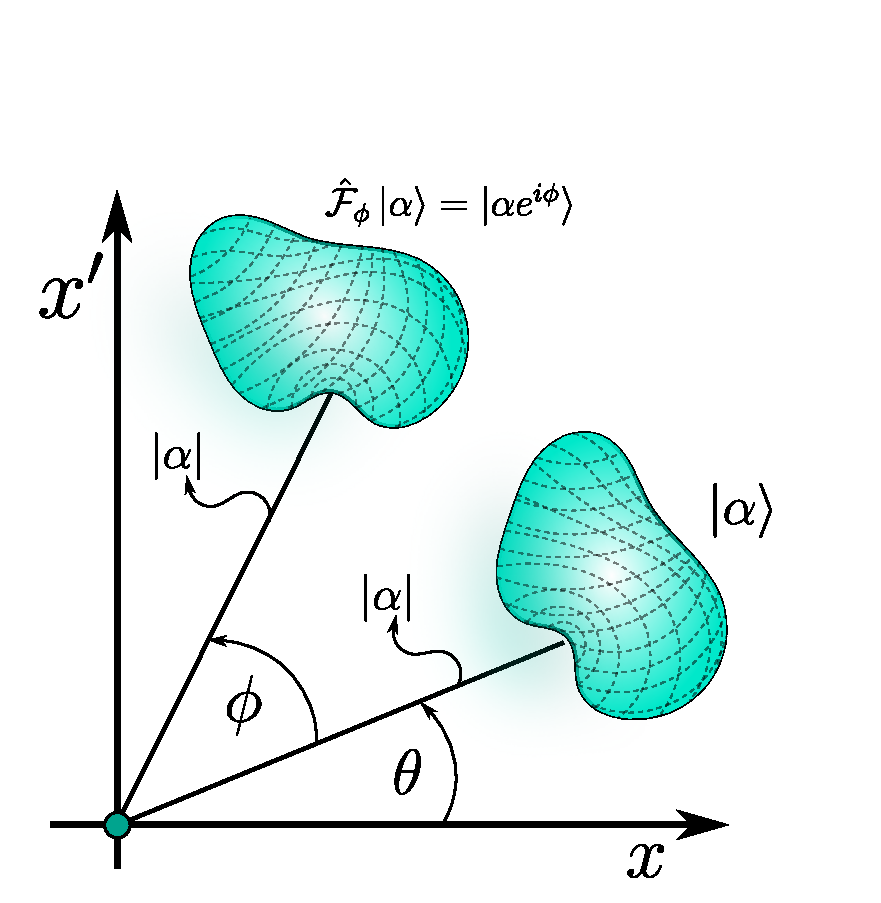
\includegraphics[width=0.75\linewidth]{Capitulo 7/Figuras/WignerRot.pdf}
            \caption{Efecto de la TFF sobre la distribución de Wigner en el espacio de fase de los estados coherentes $\ket{\alpha}$.}
            \label{fig:WignerRot}
        \end{figure}

        El interés principal para estudiar la TFF en el contexto de la fase cuántica es debido a su clara relación con los estados de fase  $\ket{\phi}$. Primero, vamos a definir los estados de fase cero como

        \begin{equation}
            \ket{\#} = \sum_{n=0}^\infty \ket{n},
        \end{equation}
        en donde podemos ver que si aplicamos la TFF sobre los estados de fase cero daremos lugar a los estados de fase como sigue

        \begin{equation}
            \hat{\mathcal{F}}_\phi \ket{\#} = e^{i\hat{N}\phi}\sum_{n=0}^{\infty}\ket{n} = \sum_{n=0}^\infty e^{in\phi}\ket{n} = \ket{\phi},
        \end{equation}
        entonces los estados $\ket{\#}$ y $\ket{\phi}$ son pares de una TFF (ver figura \ref{fig:PhaseRot}), por ende, la TFF produce una rotación de los estados de fase, esto es 

        \begin{equation}
            \hat{\mathcal{F}}_{\pm\theta}\ket{\phi} = \ket{\phi \pm \theta}.
        \end{equation}

        \begin{figure}[htbp]
            \centering
            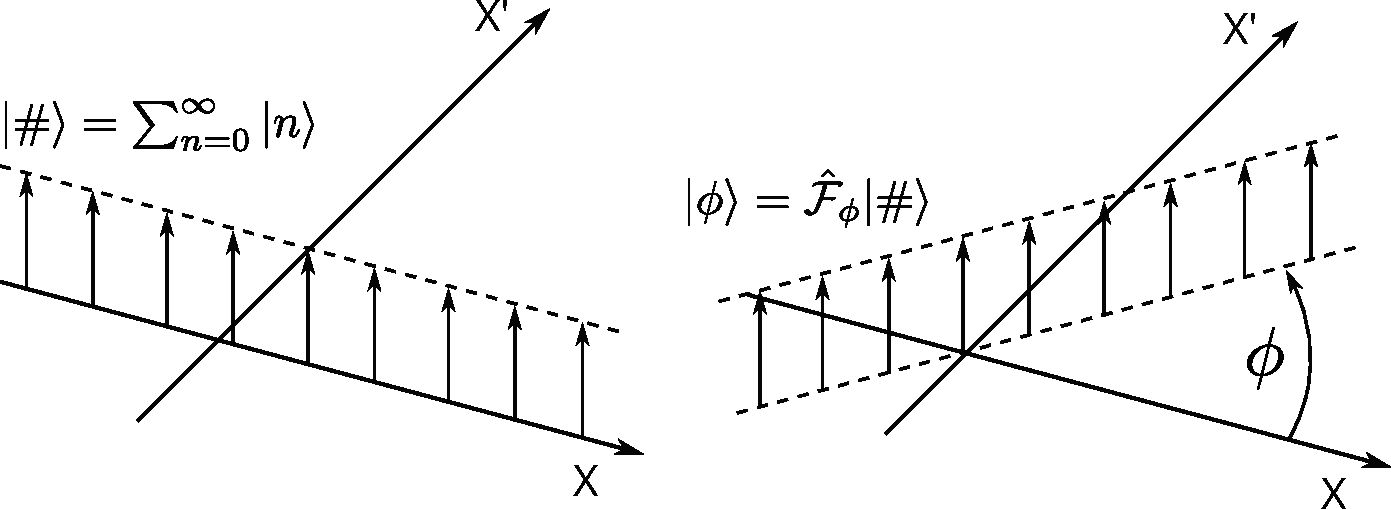
\includegraphics[width=\linewidth]{Capitulo 7/Figuras/PhaseRot.pdf}
            \caption{Representación gráfica de los estados de fase como la rotación de los estados numeral $\ket{\#}$}
            \label{fig:PhaseRot}
        \end{figure}

        Los estados de fase no forman una base ortogonal ya que un estado es deducido del otro por una rotación en el espacio de fase.

\section{Operador Exponencial de fase}

        Del operador exponencial de fase de Susskind-Glogower \ref{eq:SGNum} podemos ir definiendo las potencias del operador $\hat{E}$ de la siguiente manera

        \begin{align}
            & \hat{E}^2 = \sum_{n,n'=0}^\infty \ket{n}\braket{n+1|n'}\bra{n'+1} = \sum_{n,n'=0}^\infty\ket{n}\delta_{n'n+1}\bra{n'+1} = \sum_{n=0}^\infty \ket{n}\bra{n+2},\\
            & \hat{E}^{\dagger 2} = \sum_{n=0}^\infty \ket{n+2}\bra{n},
        \end{align}
        y, por inducción matemática, podemos probar que para cualquier $m \in \mathbb{Z}^+$ se cumple

        \begin{align}
            & \hat{E}^m = \sum_{n=0}^\infty \ket{n}\bra{n+m},\\
            & \left( \hat{E}^\dagger \right)^m = \sum_{n=0}^\infty \ket{n+m}\bra{n}.
        \end{align}

        Si tratamos de revisar la unitaridad del operador $\hat{E}^m$ vamos a llegar a una relación similar a la que se obtuvo con el operador de Susskind y Glogower, esto lo podemos demostrar de la siguiente manera

        \begin{align}\label{eq:VariosE}
            & \hat{E}^m \left( \hat{E}^\dagger \right)^m = \sum_{n,n'=0}^\infty \ket{n}\braket{n+m|n'+m}\bra{n'} = \sum_{n,n'=0}^\infty \ket{n}\delta_{nn'}\bra{n'} = \sum_{n=0}^\infty \ket{n}\bra{n}=\mathbb{I},\\
            & \left( \hat{E}^\dagger \right)^m \hat{E}^m = \sum_{n,n'=0}^\infty \ket{n+m}\braket{n|n'}\bra{n'+m} = \sum_{n,n'=0}^\infty\ket{n+m}\delta_{nn'}\bra{n'+m} = \mathbb{I}- \sum_{n=0}^{m-1}\ket{n}\bra{n},\\
            & \left[ \hat{E}^m, \left( \hat{E}^\dagger \right)^m \right] = \sum_{n=0}^{m-1}\ket{n}\bra{n},\\
            & \hat{E}^{-m} = \sum_{n=m}^\infty \ket{n}\bra{n-m} = \sum_{n=0}^\infty \ket{n+m}\bra{n} = \left( \hat{E}^\dagger \right)^m.
        \end{align}

        De lo anterior tenemos que el operador $\hat{E}^m$ es también semi-unitario, como se esperaría ya que este proviene del operador exponencial de fase de Susskind y Glogower, el cual ya era semi-unitario. Lo interesante está en que, mientras que para $m=1$, si $n$ es muy grande, el operador es aproximadamente unitario ya que el efecto del vacío cuántico puede llegar a ser despreciable, sin embargo, para el operador $\hat{E}^m$ podemos observar que esto no es válido, incluso cuando $m \to \infty$ el operador $\left( \hat{E}^\dagger \right)^m$ será ortogonal por izquierda al operador $\hat{E}^m$.

        Antes de seguir, es útil evaluar los siguientes conmutadores entre el exponencial de fase y el operador TFF como sigue

        \begin{align}
            & \left[ \hat{E}^m, \hat{\mathcal{F}}_\theta \right] = \sum_{n=0}^\infty \ket{n}\bra{n+m}\hat{\mathcal{F}}_\theta - \hat{\mathcal{F}}_\theta \sum_{n=0}^\infty \ket{n}\bra{n+m},\\
            & \left[ \hat{E}^m, \hat{\mathcal{F}}_\theta \right] = \sum_{n=0}^{\infty} e^{i(n+m)\theta}\ket{n}\bra{n+m} - \sum_{n=0}^{\infty} e^{in\theta} \ket{n}\bra{n+m},\\
            & \left[ \hat{E}^m, \hat{\mathcal{F}}_\theta \right] = \left( e^{im\theta} -1 \right)\sum_{n=0}^\infty e^{in\theta}\ket{n}\bra{n+m} = \left( e^{im\theta}-1 \right)\hat{\mathcal{F}}_\theta\hat{E}^m.
        \end{align}
        Con el operador adjunto conjugado tenemos una relación semejante

        \begin{equation}
            \left[ \left( \hat{E}^\dagger \right)^m, \hat{\mathcal{F}}_\theta \right] = \left( 1-e^{im\theta} \right)\left( \hat{E}^\dagger \right)^m \hat{\mathcal{F}}_\theta.
        \end{equation}

        De estas dos últimas relaciones de conmutación podemos llegar a las siguientes ecuaciones

        \begin{equation}
            \hat{\mathcal{F}}_\theta \left( \hat{E}^\dagger \right)^m \hat{\mathcal{F}}_\theta^\dagger = \left( \hat{E}^\dagger \right)^me^{im\theta}, \quad \hat{\mathcal{F}}_\theta \hat{E}^m \hat{\mathcal{F}}^\dagger_\theta = \hat{E}^m e^{-im\theta},
        \end{equation}
        y si aplicamos estos operadores sobre los estados de fase $\ket{\phi}$ tendremos

        \begin{equation}\label{eq:FFSimil}
            \hat{\mathcal{F}}_\theta \hat{E}^m \hat{\mathcal{F}}^\dagger_\theta \ket{\phi} = e^{im(\phi-\theta)}\ket{\phi}, \quad \hat{\mathcal{F}}_\theta \left( \hat{E}^\dagger \right)^m \hat{\mathcal{F}}_\theta^\dagger\ket{\phi} = e^{-im(\phi-\theta)}\ket{\phi}.
        \end{equation}

        En las ecuaciones \ref{eq:FFSimil} observamos que la transformación de similaridad de los operadores exponencial de fase en términos de la TFF nos lleva a un cambio de espacio de fase donde el estado de fase cero se ha modificado por $\phi = \theta$.

\section{Operador de fase cuántica}

        Con base en los estados numeral, podemos definir su proyector en los estados de fase cero como sigue

        \begin{equation}
            \ket{\#}\bra{\#} = \sum_{n,n'=0}^\infty \ket{n}\bra{n'} = \sum_{m=-\infty}^\infty \hat{E}^m
        \end{equation}
        y utilizando las ecuaciones \ref{eq:VariosE} tendremos
        \begin{equation}
            \ket{\#}\bra{\#} = \sum_{n=0}^\infty \ket{n}\bra{n} + \sum_{m=1}^\infty \left[ \hat{E}^m + \left( \hat{E}^\dagger \right)^m \right],
        \end{equation}
        entonces el operador proyector de fase será

        \begin{equation}
            \ket{\theta}\bra{\theta} = \hat{\mathcal{F}}_\theta \ket{\#}\bra{\#}\hat{\mathcal{F}}_\theta^\dagger = \sum_{n=0}^\infty \ket{n}\bra{n} + \sum_{m=1}^\infty \left[ \hat{\mathcal{F}}_\theta \hat{E}^m \hat{\mathcal{F}}_\theta^\dagger + \hat{\mathcal{F}}_\theta \left( \hat{E}^\dagger \right)^m \hat{\mathcal{F}}_\theta^\dagger \right],
        \end{equation}
        y usando las relaciones de similaridad encontradas en \ref{eq:FFSimil} tenemos que el proyector de fase es

        \begin{equation}\label{eq:FaseProy}
            \ket{\theta}\bra{\theta} = \sum_{n=0}^\infty\ket{n}\bra{n} + \sum_{m=1}^\infty \left[ \hat{E}^m e^{-im\theta} + \left( \hat{E}^\dagger \right)^me^{im\theta} \right].
        \end{equation}

        Vale la pena mencionar que el proyector $\hat{P}_\theta = \ket{\theta}\bra{\theta}$ al no conmutar con $\hat{E}^m$ hace que los estados de fase $\ket{\phi}$ no sean estados propios de $\hat{P}_\theta$.

        Debido a que los estados de fase no son ortogonales, vamos a adoptar la formulación de operadores Hermíticos de Toeplitz-Rosenblum \cite{rosenblum1962self}. Entonces para un $f: \Omega \subseteq \mathbb{R} \to \mathbb{R}$ una función Lebesgue-integrable, un operador hermítico puede ser definido en la forma

        \begin{equation}
            \hat{F}_\phi = \frac{1}{2\pi}\int_\phi ^{\phi + 2\pi} f(\theta) \ket{\theta}\bra{\theta}d\theta,
        \end{equation}
        para $f(\theta) = \theta$, tenemos el operador de Garrison y Wong \cite{garrison1970canonically}, y usando el proyector \ref{eq:FaseProy} tenemos

        \begin{align}
            & \hat{\Theta}_\phi = \frac{1}{2\pi}\int_\phi^{\phi+2\pi}\theta\ket{\theta}\bra{\theta}d\theta,\\
            & \hat{\Theta}_\phi = \sum_{n=0}^\infty \ket{n}\bra{n}\frac{1}{2\pi}\int_\phi^{\phi+2\pi} \theta d\theta + \sum_{m=1}^\infty \hat{E}^m\frac{1}{2\pi}\int_{\phi}^{\phi+2\pi}\theta e^{-im\theta}d\theta + \sum_{m=1}^\infty \left( \hat{E}^\dagger \right)^m \frac{1}{2\pi}\int_\phi^{\phi+2\pi}\theta e^{im\theta}d\theta,
        \end{align}
        usando
        \begin{equation}
            \frac{1}{2\pi}\int_{\phi}^{\phi+2\pi} \theta e^{\pm im\theta}d\theta = \mp \frac{i}{m}e^{\pm im\phi},
        \end{equation}
        entonces

        \begin{align}
            & \hat{\Theta}_\phi = (\phi+\pi) \sum_{n=0}^\infty \ket{n}\bra{n} + i \sum_{m=1}^\infty \frac{e^{-im\phi}}{m}\sum_{n=0}^\infty \ket{n}\bra{n+m} - i \sum_{m=1}^\infty \frac{e^{im\phi}}{m}\sum_{n=0}^\infty \ket{n+m}\bra{n}.
        \end{align}

        Antes de seguir, debemos tener en cuenta las siguientes ecuaciones

        \begin{align}
            & \hat{\mathcal{F}}_\phi \ket{n}\bra{n+m}\hat{\mathcal{F}}_\phi^\dagger = e^{-im\phi}\ket{n}\bra{n+m},\\
            & \hat{\mathcal{F}}_\phi \ket{n+m}\bra{n}\hat{\mathcal{F}}_\phi^\dagger = e^{im\phi}\ket{n+m}\bra{n},
        \end{align}
        entonces, finalmente, el operador Hermítico de fase se define como

        \begin{equation}
            \hat{\Theta}_\phi = (\phi + \pi) \sum_{n=0}^\infty \ket{n}\bra{n} + \hat{\mathcal{F}}_\phi \left[ \sum_{n=0}^\infty\sum_{m=1}^\infty i \frac{\ket{n}\bra{n+m} - \ket{n+m}\bra{n}}{m} \right]\hat{\mathcal{F}}_\phi^\dagger,
        \end{equation}
        y para el caso $\phi = - \pi$ tenemos
        \begin{equation}
            \hat{\Theta}_{-\pi} = \sum_{n=0}^\infty \sum_{m=1}^\infty \frac{i^{2m+1}}{m}\left( \ket{n}\bra{n+m} - \ket{n+m}\bra{n} \right).
        \end{equation}

        Debido a que los estados $\ket{\phi}$ no son ortogonales, el cuadrado del operador $\hat{\Theta}_\phi$ no puede ser formulado mediante potencias, sino que este se debe calcular mediante la formulación de Toeplitz-Rosenblum para $f(\theta) = \theta^2$, entonces

        \begin{align}
            & \hat{\Theta}_\phi^2 = \frac{1}{2\pi}\int_\phi^{\phi+2\pi} \theta^2 \ket{\theta}\bra{\theta}d\theta,\\
            & \hat{\Theta}_\phi^2 = \sum_{n=0}^\infty \ket{n}\bra{n}\frac{1}{2\pi}\int_\phi^{\phi+2\pi}\theta^2 d\theta + \sum_{m=1}^\infty \hat{E}^m \frac{1}{2\pi}\int_\phi^{\phi+2\pi} \theta^2 e^{-im\theta}d\theta + \sum_{m=1}^\infty\left( \hat{E}^\dagger \right)^m\frac{1}{2\pi}\int_\phi^{\phi+2\pi}\theta^2e^{im\theta}d\theta,
        \end{align}
        usando el siguiente resultado del cálculo integral
        \begin{equation}
            \frac{1}{2\pi}\int_\phi^{\phi+2\pi}\theta^2 e^{\pm im\theta}d\theta = 2 \left[ \frac{\mp i (\phi+\pi)}{m}+ \frac{1}{m^2} \right]e^{\pm i m\phi},
        \end{equation}
        entonces
        \begin{align}
            & \hat{\Theta}_\phi^2 = \left[ (\phi+\pi)^2 + \frac{\pi^2}{3} \right]\sum_{n=0}^\infty\ket{n}\bra{n} + 2(\phi+\pi)\hat{\mathcal{F}}_\phi \left[ \sum_{n=0}^\infty\sum_{m=1}^\infty i \frac{\ket{n}\bra{n+m} -\ket{n+m}\bra{n} }{m} \right]\hat{\mathcal{F}}_\phi^\dagger\\
            &  + 2\hat{\mathcal{F}}_\phi \left[ \sum_{n=0}^\infty\sum_{m=1}^\infty \frac{\ket{n}\bra{n+m} + \ket{n+m}\bra{n}}{m^2} \right]\hat{\mathcal{F}}_\phi^\dagger.
        \end{align}

        Como el ángulo inicial $\phi$ es arbitrario, podemos escoger a $\phi = -\pi$, entonces

        \begin{equation}
            \hat{\Theta}_{-\pi}^2 = \frac{\pi^2}{3}\sum_{n=0}^\infty \ket{n}\bra{n} + 2 \left[ \sum_{n=0}^\infty\sum_{m=1}^\infty \frac{i^{2m}}{m^2}\left(  \ket{n}\bra{n+m} + \ket{n+m}\bra{n} \right)\right].
        \end{equation}

        London \cite{london1926jacobischen,london1927winkelvariable} mostró que la fase y el número de fotones no están asociados con operadores canónicamente conjugados cuya relación de incertidumbre no puede ser formulado en términos de los operadores de posición y momento dados. En este orden de ideas, calculamos el conmutador $\left[ \hat{N},\hat{\Theta} \right]$ entonces

        \begin{align}
            & \hat{N}\hat{\Theta} = \sum_{k=0}^\infty k \ket{k}\bra{k} \sum_{n=0}^\infty \sum_{m=1}^\infty  \frac{i^{2m+1}}{m}\left( \ket{n}\bra{n+m} - \ket{n+m}\bra{n} \right),
        \end{align}


        \begin{align}
            & \hat{N}\hat{\Theta} = \sum_{n=0}^\infty\sum_{m=1}^\infty \frac{i^{2m+1}}{m}\left( n\ket{n}\bra{n+m} - (n+m)\ket{n+m}\bra{n} \right),\\
            & \hat{N}\hat{\Theta} = \sum_{n=0}^\infty\sum_{m=1}^\infty\frac{i^{2m+1}n}{m}\left( \ket{n}\bra{n+m} - \ket{n+m}\bra{n}\ \right) - \sum_{n=0}^\infty\sum_{m=1}^\infty i^{2m+1}\ket{n+m}\bra{n},
        \end{align}
        similarmente
        \begin{equation}
            \hat{\Theta}\hat{N}= \sum_{n=0}^\infty\sum_{m=1}^\infty \frac{i^{2m+1}n}{m} \left( \ket{n}\bra{n+m}-\ket{n+m}\bra{n} \right) + \sum_{n=0}^\infty \sum_{m=1}^\infty i^{2m+1}\ket{n}\bra{n+m},
        \end{equation}
        por ende el conmutador entre el número de fotones y el operador de fase será

        \begin{equation}
            \left[ \hat{N},\hat{\Theta} \right] = -i \sum_{n=0}^\infty\sum_{m=1}^\infty (-1)^m \left( \ket{n}\bra{n+m} + \ket{n+m}\bra{n} \right),
        \end{equation}
        con $\phi = -\pi$ tenemos
        \begin{equation}
            \sum_{n=0}^\infty\sum_{m=1}^\infty(-1)^m \left( \ket{n}\bra{n+m} + \ket{n+m}\bra{n} \right) = \ket{\pi}\bra{\pi} - \mathbb{I},
        \end{equation}
        finalmente el conmutador será

        \begin{equation}
            \left[ \hat{N},\hat{\Theta} \right] = i \left( \mathbb{I} - \ket{\pi}\bra{\pi} \right),
        \end{equation}
        donde el operador $\ket{\pi}\bra{\pi}$ corresponde a la función singular $\delta(\theta-\pi)$ (ver figura \ref{fig:chivsphi}). Entonces tenemos una relación de conmutación en la forma postulada por Judge y Lewis \cite{judge1963commutator}, donde $\hat{\Theta}$ es expresada como una función $2\pi$ periódica pero para nuestro caso de los operadores número y fase sin la necesidad de introducir operadores número negativos o espacios de Hilbert extendidos. 
\section{El operador de diferencia de fase cuántica y su relación con la polarización}

    Otra de las diferentes propuestas respecto a la formulación de la fase es la desarrollada por Alfredo Luis y Luis Sanchez Soto \cite{Diferencia-Fase}. En su artículo, resaltan el hecho de que la mayor parte del trabajo invertido en este problema se enfoca principalmente en las propiedades de un operador de fase para el campo electromagnético con un único modo de oscilación. Sin embargo, en un sentido práctico la noción de fase recupera mayor relevancia si se trata de una diferencia de fase entre una oscilación y otra que se tome de referencia, siendo esta una motivación para introducir lo que denominan un operador de diferencia de fase. \\ 
    
    
    En este sentido, se considera nuevamente un operador exponencial de fase $\hat{E}_{12}$, el cual ahora va a estar definido para un estado bimodal de campo $|n_1,n_2\rangle$, para lo cual se efectúa la descomposición polar 
    
    \begin{equation}
    \widehat{a}_{1}\widehat{a}^{\dagger}_2 = \hat{E}_{12}\sqrt{\hat{N}_1(\hat{N}_2 + 1)}.
    \end{equation}
    
    Sin embargo, esta relación no logra caracterizar por completo al operador $\hat{E}_{12}$, pues por ejemplo si deseamos estudiar el caso en el que la totalidad de fotones se encuentra en sólo uno de los modos, encontramos que los elementos de $\langle n_1,0| \hat{E}_{12} | 0,n_2\rangle$ no están definidos. Por lo que es necesario caracterizar otras condiciones para el operador, las cuales pueden ser obtenidas mediante la relación de conmutación con la acción $j$ del oscilador armónico, la cual puede entenderse como un momento angular. Para ello, clásicamente se sabe que satisface el corchete de Poisson
    
    \begin{equation}\label{eq:Poisson1}
        \{j,\phi\} = 1,
    \end{equation}
    y
    \begin{equation}\label{eq:Poisson2}
        \{j_1 + j_2,\phi_{12}\} = 0,
    \end{equation}
    \begin{equation}
        \left\{\frac{j_1 - j_2}{2},\phi_{12}\right\} = 1
    \end{equation}
    para el caso de dos osciladores independientes. De manera que para nuestros osciladores cuánticos tendríamos 
    \begin{equation}
        [E_{12},N_1+N_2] = 0,
    \end{equation}
    y 
    \begin{equation}
        \left[E_{12},\frac{N_1 - N_2}{2}\right] = E_{12}.
    \end{equation}
    Esta segunda ecuación se puede interpretar como el análogo al criterio de Lerner.

    Debe notarse que hay una solución no unitaria para $\hat{E}_{12}$ que verifica simultáneamente estas dos relaciones de conmutación y se le puede llamar como el operador exponencial de diferencia de fase de Susskind-Glogower. La falta de unitaridad de esta solución es un remanente de la incompatibilidad con una traducción cuántica de los corchetes de Poisson \ref{eq:Poisson1},\ref{eq:Poisson2}.

    Para proponer un operador de diferencia de fase vamos a tomar ventaja de que los siguientes operadores
    \begin{align}\label{eq:Jotas}
        & \hat{J}_x = \frac{1}{2}\left(  \hat{a}_1^\dagger \hat{a}_2 + \hat{a}_2^\dagger\hat{a}_1\right),\\
        & \hat{J}_y = \frac{i}{2}\left( \hat{a}_2^\dagger\hat{a}_1 - \hat{a}_1^\dagger\hat{a}_2 \right),\\
        & \hat{J}_z = \frac{1}{2}\left( \hat{a}_1^\dagger \hat{a}_1 - \hat{a}_2^\dagger\hat{a}_2 \right),
    \end{align}
    satisfacen las relaciones de conmutación del álgebra de Lie del grupo de rotaciones tridimensionales $SU(2)$:
    \begin{equation}
        \left[ \hat{J}_k, \hat{J}_l \right] = i \epsilon_{klm}\hat{J}_m.
    \end{equation}
    El invariante de Casimir para este grupo puede ser puesto en la forma
    \begin{equation}
        \hat{J}^2 = \frac{\hat{N}}{2}\left( \frac{\hat{N}}{2}+1 \right);
    \end{equation}
    de hecho, $\hat{N}$ conmuta con todos los operadores $\hat{J}_i\;,\; i=1,2,3$. El espacio de Hilbert total del problema $\mathcal{H}_1\otimes \mathcal{H}_2$ puede ser expresado como una suma directa de los subespacios invariantes bajo los operadores de momento angular
    \begin{equation}
        \mathcal{H}_1\otimes\mathcal{H}_2 = \bigoplus_{n=0}^\infty \mathcal{H}_n.
    \end{equation}

    Cada $\mathcal{H}_n$ tiene un número total de fotones $n$ fijo y es generado por los $2j+1=n+1$ vectores $\ket{j,m}$, los cuales son estados propios en común de $\hat{J}^2$ y $\hat{J}_z$. Los estados propios de número $\ket{n_1,n_2}\in \mathcal{H}_n$ corresponden a la base $\ket{j,m}$ como sigue

    \begin{equation}
        \ket{n_1,n_2} = \ket{j = (n_1+n_2)/2, m = (n_1-n_2)/2}.
    \end{equation}

    Podemos definir unos operadores escalera de momento angular $\hat{J}_\pm$ tales que

    \begin{align}
        & \hat{J}_+ = \hat{J}_x + i \hat{J}_y = \hat{a}_1^\dagger\hat{a}_2,\\
        & \hat{J}_- = \hat{J}_x -i\hat{J}_y = \hat{a}_1\hat{a}_2^\dagger,
    \end{align}
    en donde podemos ver la relación entre $\hat{J}_\pm$ y el operador exponencial de diferencia de fase $\hat{E}_{12}$ como

    \begin{equation}\label{eq:JE12}
        \hat{J}_- = \hat{E}_{12}\sqrt{\hat{J}_+\hat{J}_-}.
    \end{equation}

    Debido a que el operador $\hat{E}_{12}$ conmuta con el número total de fotones $\hat{N}$ entonces vamos a restringir un poco el estudio a cada subespacio $\mathcal{H}_n$ y, posteriormente, extender esto al espacio de Hilbert completo. Sea $\hat{E}_{12}^{(n)}$ la restricción, entonces la ecuación \ref{eq:JE12} se puede resolver obteniendo el operador exponencial de diferencia de fase unitario $SU(2)$ como

    \begin{equation}\label{eq:E12Jotas}
        \hat{E}_{12}^{(n)} = \sum_{m=-j+1}^j \ket{j,m-1}\bra{j,m}+e^{i(n+1)\phi^{(n)}}\ket{j,j}\bra{j,-j},
    \end{equation}
    siendo $\phi^{(n)}$ una fase arbitraria. Nótese que el término extra en \ref{eq:E12Jotas} es importante ya que garantiza la unitaridad de $\hat{E}_{12}^{(n)}$ y se sostiene en la finitud de los estados número. Para los operadores del oscilador armónico tal descomposición es inviable porque sus estados número se extienden hacia el infinito y no tiene un término extra que proyecte un estado superior a un estado base ( a menos de que uno decida truncar como en el formalismo de Pegg-Barnett). De esta manera, en cada subespacio $\mathcal{H}_n$ hay $n+1$ estados ortonormales que verifican

    \begin{equation}
        \hat{E}_{12}^{(n)}\ket{\phi_r^{(n)}} = e^{i\phi_r^{(n)}}\ket{\phi_r^{(n)}},
    \end{equation}
    con $r=0,...,n.$ Estos estados se pueden expresar en la base de los estados número como

    \begin{equation}
        \ket{\phi_r^{(n)}} = \frac{1}{\sqrt{n+1}} \sum_{n_1=0}^n e^{in_1\phi_r^{(n)}}\ket{n_1,n-n_1},
    \end{equation}
    donde, al tomar la misma ventana de $2\pi$ en cada subespacio, tenemos
    \begin{equation}
        \phi_r^{(n)} = \phi_0 + \frac{2\pi r}{n+1}.
    \end{equation}

    La expresión para $\hat{E}_{12}$ en todo el espacio se obtiene al tomar las infinitas copias del exponencial de diferencia de fase de $SU(2)$
    \begin{align}
        & \hat{E}_{12} = \sum_{n=0}^\infty \hat{E}_{12}^{(n)} = \sum_{n=0}^\infty \sum_{r=0}^n \ket{\phi_r^{(n)}}e^{i\phi_r^{(n)}}\bra{\phi_r^{(n)}},\\
        & \hat{E}_{12} = \sum_{n=0}^\infty \frac{1}{n+1}\sum_{r=0}^n \sum_{k,k'=0}^n \ket{k,n-k}e^{i\left( k-k'+1 \right)\phi_r^{(n)}}\bra{k',n-k'}.
    \end{align}

    Como $\hat{E}_{12}$ es unitario, este define un operador de diferencia de fase hermítico
    \begin{equation}
        \hat{\phi}_{12} = \sum_{n=0}^\infty \sum_{r=0}^n \ket{\phi_r^{(n)}}\phi_r^{(n)}\bra{\phi_r^{(n)}},
    \end{equation}
    y finalmente tenemos $\hat{E}_{12} = e^{i\hat{\phi}_{12}}$.

    Este operador difiere de otros, principalmente porque no se puede obtener de una construcción previa de los operadores de fase para cada uno de los osciladores individuales involucrados. Además, a diferencia del formalismo de Susskind-Glogower, $\hat{E}_{12}$ así definido sí es unitario.

    A su vez, el espectro de valores propios de $\hat{\phi}_{12}$ es discreto, para cada subespacio $\mathcal{H}_n$ hay $n+1$ uniformemente distribuidos valores propios en el intervalo $[0,2\pi]$, a diferencia de otros formalismos que dan un espectro continuo en el intervalo $[0,4\pi]$.

    Podemos dar una interpretación física a los operadores de momento angular y al operador de diferencia de fase en términos de la polarización. Una forma de lidiar con la polarización a nivel cuántico es con los operadores de Stokes definidos por

    \begin{align}
        &\hat{S}_0 = \hat{a}_1^\dagger\hat{a}_1 + \hat{a}_2^\dagger\hat{a}_2,\\
        & \hat{S}_1 = \hat{a}_1^\dagger\hat{a}_2 + \hat{a}_2^\dagger\hat{a}_1,\\
        & \hat{S}_2 = i\left( \hat{a}_2^\dagger\hat{a}_1 - \hat{a}_1^\dagger\hat{a}_2 \right),\\
        & \hat{S}_3 = \hat{a}_1^\dagger \hat{a}_1 - \hat{a}_2^\dagger \hat{a}_2.
    \end{align}

    Nótese que, excepto por un factor de $2$, los operadores $\hat{S}_i\;,\; i=1,2,3$ coinciden con los operadores \ref{eq:Jotas} de momento angular, mientras que $\hat{S}_0$ representa el número total de fotones $\hat{N}$. La no conmutatividad de los operadores de Stokes nos advierte sobre la imposibilidad de hacer mediciones simultáneas de las cantidades físicas asociadas a estos operadores. Los operadores $\hat{S}_i$ pueden ser vistos como generadores de un grupo de transformaciones localmente isomorfas al grupo de rotaciones tridimensional que dejan invariante al operador $\hat{S}_0$.

    Estos operadores de Stokes replican los parámetros de Stokes cuando calculamos los valores medios en la base de los estados coherentes bimodales dados por
    \begin{equation}
        \ket{\alpha_1,\alpha_2} = e^{-\frac{|\alpha_1|^2+|\alpha_2|^2}{2}}\sum_{n_1,n_2=0}^\infty \frac{\alpha_1^{n_1}\alpha_2^{n_2}}{\sqrt{n_1! n_2!}}\ket{n_1,n_2},
    \end{equation}
    en donde los parámetros de Stokes se calculan como

    \begin{align}
        & s_0 = \bra{\alpha_1,\alpha_2}\hat{S}_0 \ket{\alpha_1,\alpha_2} = |\alpha_1|^2 + |\alpha_2|^2,\\
        & s_1 = \bra{\alpha_1,\alpha_2}\hat{S}_1 \ket{\alpha_1,\alpha_2} = 2|\alpha_1||\alpha_2|\cos(\phi_1-\phi_2), \\
        & s_2 = \bra{\alpha_1,\alpha_2}\hat{S}_2 \ket{\alpha_1,\alpha_2} = -2|\alpha_1||\alpha_2|\sin(\phi_1-\phi_2), \\
        & s_3 = \bra{\alpha_1,\alpha_2}\hat{S}_3 \ket{\alpha_1,\alpha_2} = |\alpha_1|^2 - |\alpha_2|^2.
    \end{align} 

    Si denotamos como $s_\pm = (s_1\pm is_2)/2$ entonces la diferencia de fase clásica entre dos modos se obtiene sin ambigüedades como

    \begin{equation}
        s_+ = e^{-i(\phi_1-\phi_2)}|\alpha_1||\alpha_2| = e^{-i(\phi_1-\phi_2)}\sqrt{s_-s_+}.
    \end{equation}